% !TeX root = ../../main.tex

For a simplicial complex $K$ let $C_k(K)$ denote the vector space over a field $\FF$ consisting of linear combinations of $k$-simplices in $K$ known as \textbf{$k$-chains}.
These vector spaces are connected by \textbf{boundary maps} $\partial_k: C_k(K)\to C_{k-1}(K)$ which are linear transformations taking basis elements of $C_k(K)$ to the abstract sum of basis $(k-1)$-simplex faces.
The collection of chains and boundary maps forms a sequence of vector spaces known as the \textbf{chain complex} of $K$.
We can define a chain complex, known as the singular chain complex, in a similar way for any topological space $X$.
We will primarily be using singular homology over a field $\FF$ so that the homology groups $\hom_k(X)$ of a topological space $X$ are vector spaces.
For a full treatment of both singular and simplicial homology see Hatcher~\cite{hatcher01}.

An important property of the boundary maps $\partial_k$ is that the composition of subsequent boundary maps is zero.
That is, $\partial_k\circ\partial_{k-1} = 0$ for all $k$.
% As a result the image of $\partial_{k+1}$, denoted $\im~\partial_{k+1} = \{\partial_{k+1}c\mid c\in C_{k+1}(K)\}$ is a subspace of the kernel, $\ker~\partial_k = \{c\in C_k(K)\mid \partial_k c = 0\}$, of $\partial_k$.
As a result the image of $\partial_{k+1}$, denoted $\im~\partial_{k+1}$ is a subspace of the kernel, $\ker~\partial_k$, of $\partial_k$.
A \textbf{$k$-cycle} is a $k$-chain with empty boundary---an element of $\ker~\partial_k$.
Two cycles in $\ker~\partial_k$ are said to be \textbf{homologous} if they differ by an element of $\im~\partial_{k+1}$.

The \textbf{$k$th homology groups} of a topological space $X$ is the quotient group $\hom_k(X) = \ker~\partial_k/\im~\partial_{k+1}$.
Elements of $\hom_k(X)$ are equivalence classes $[x]$ of homologous $k$ cycles.
That is, if $[x] = [y]$ for any $x,y\in C_k(K)$ then $x = y +\partial_{k+1}(z)$ for some $z\in C_{k+1}(X)$.

The dimension of a homology group is of particular importance and is known as a \textbf{Betti number} $\beta_k = \dim~\hom_k(X)$.
The Betti numbers are topological invariants that count equivalence classes of $k$-cycles that are \emph{not} the boundary of $(k+1)$-chains.
These equivalence classes are more often described as $k$-dimensional ``holes'' in a topological space, where $0$-dimensional holes are connected components, $1$-dimensional holes are loops, $2$-dimensional holes are voids, and so on.
The homology groups not only count these homological features but also provide a partition of the $k$-cycles into equivalence classes.
In practice, one can recover representative cycles for homology groups that have interesting geometric and topological significance.

\begin{figure}[htbp]
  \centering
  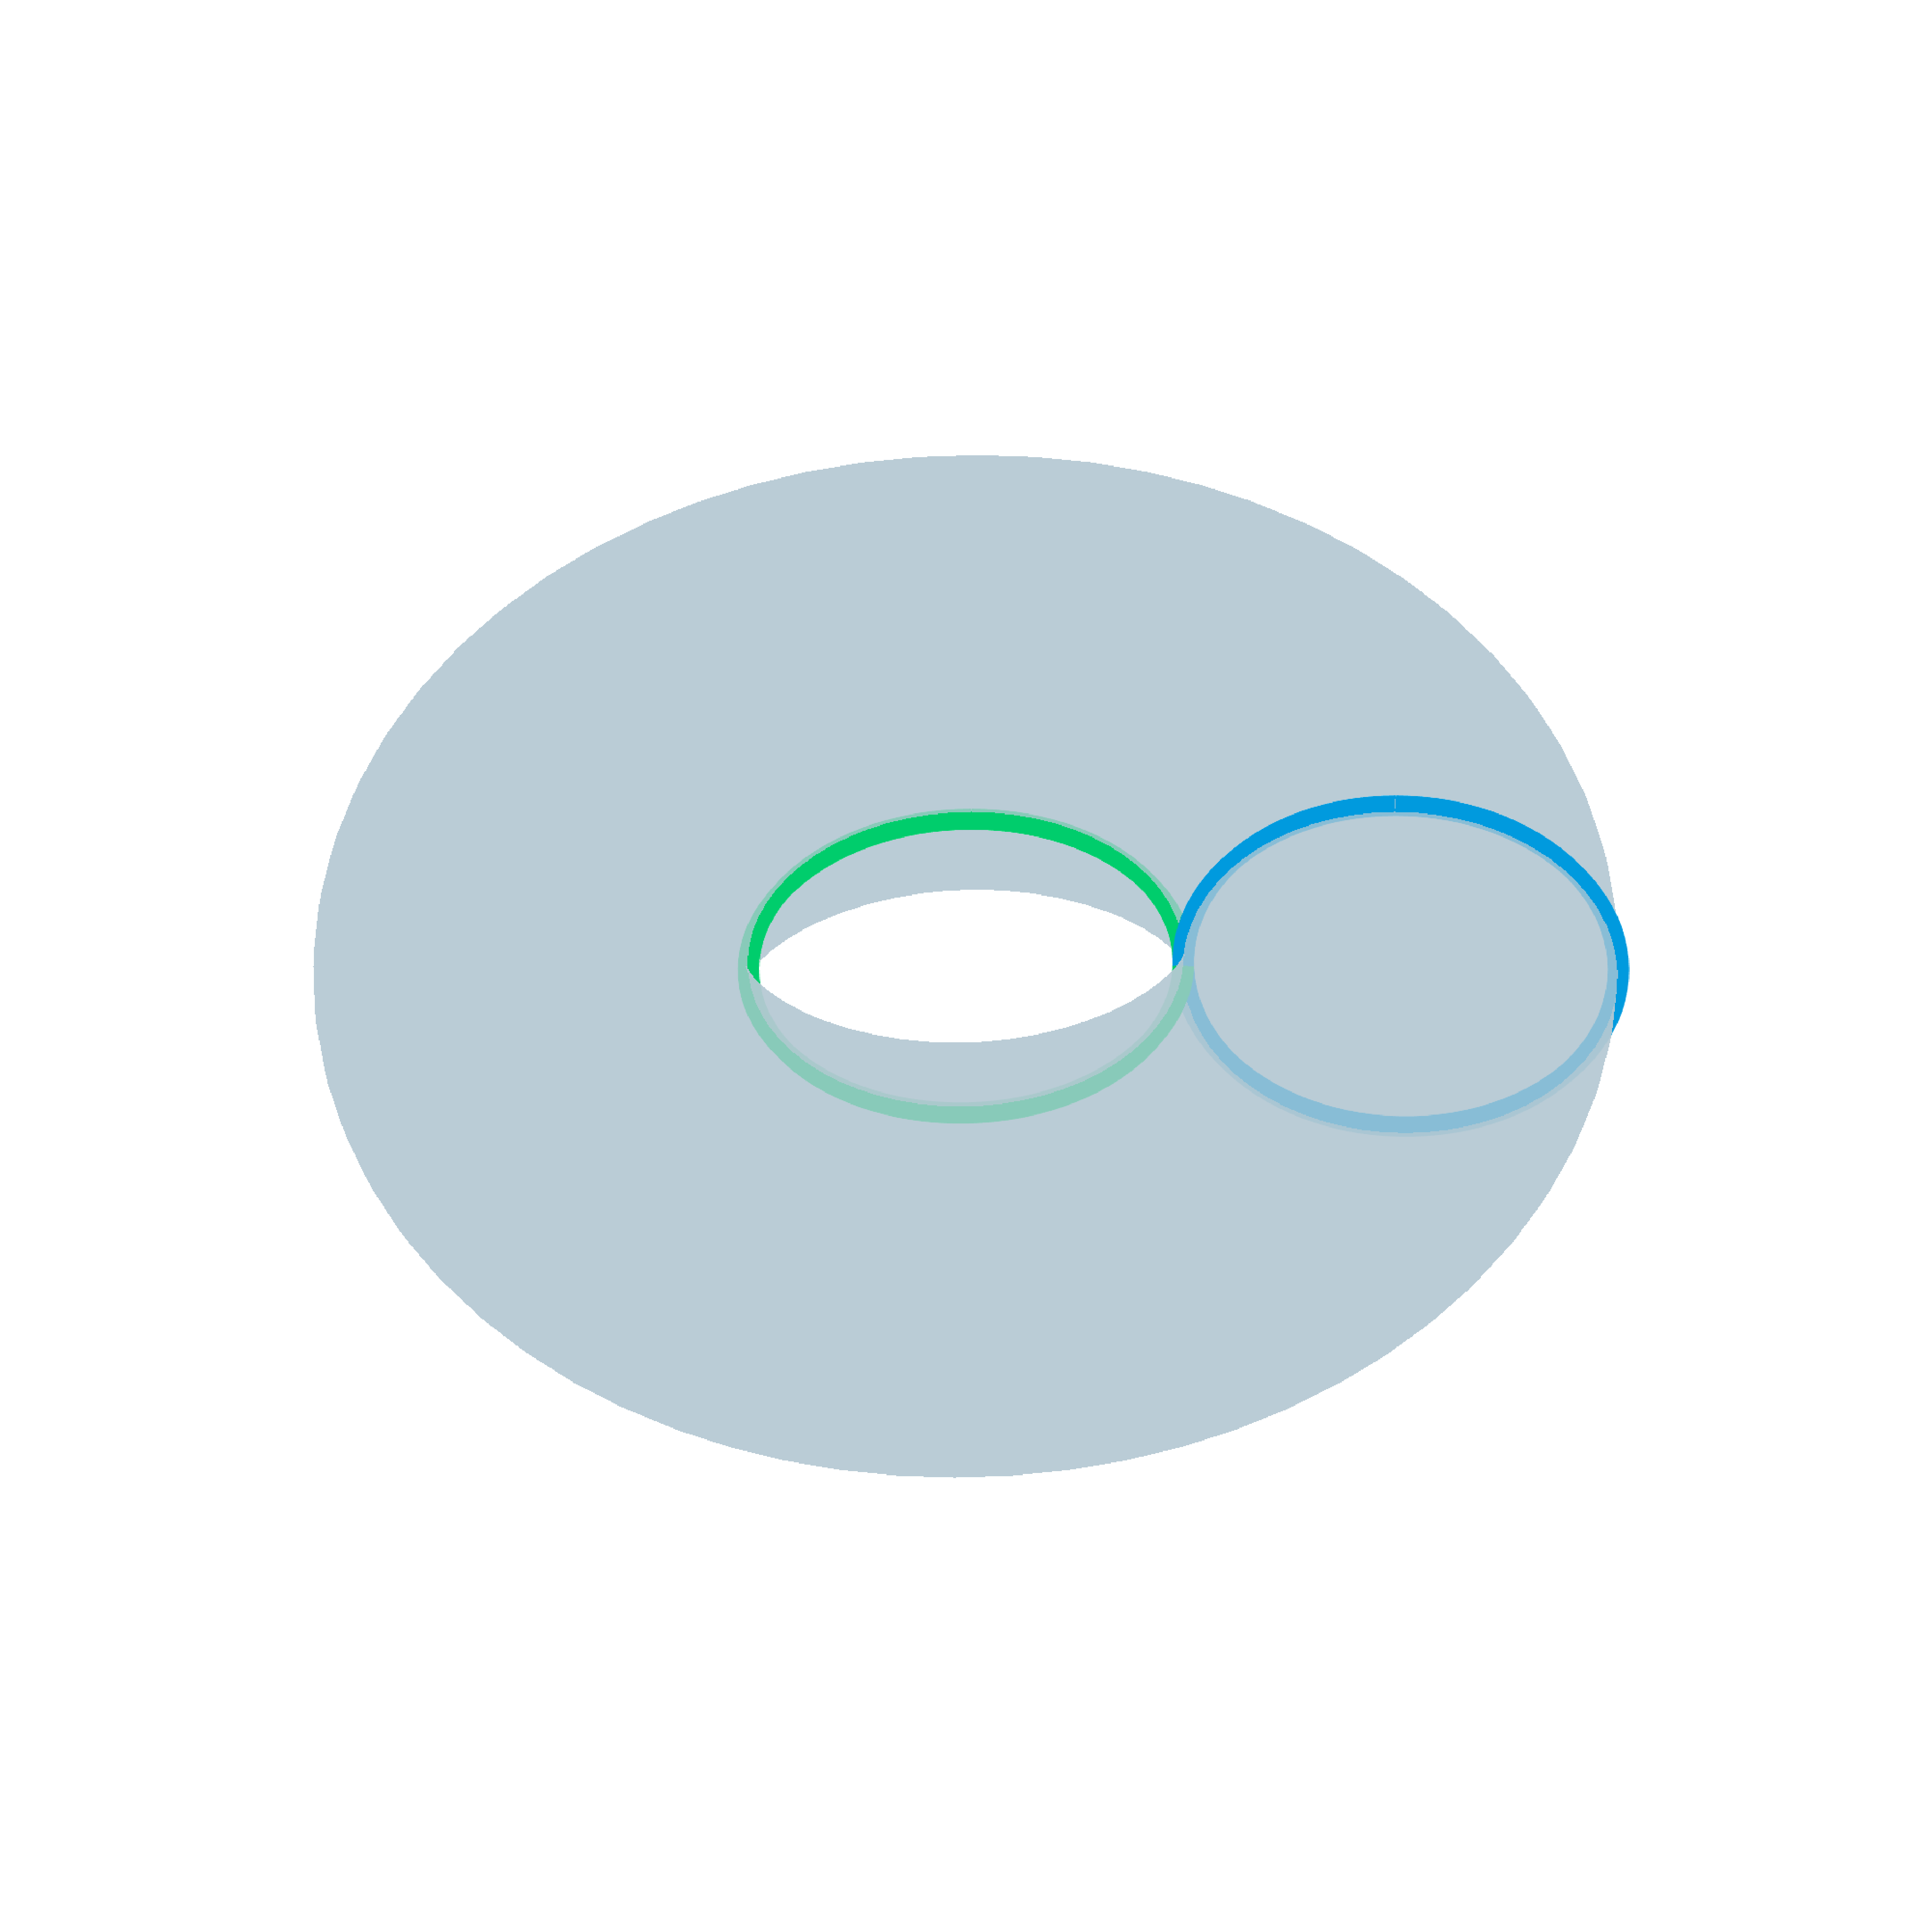
\includegraphics[trim=0 300 0 300, clip, width=0.4\textwidth]{figures/torus1}
  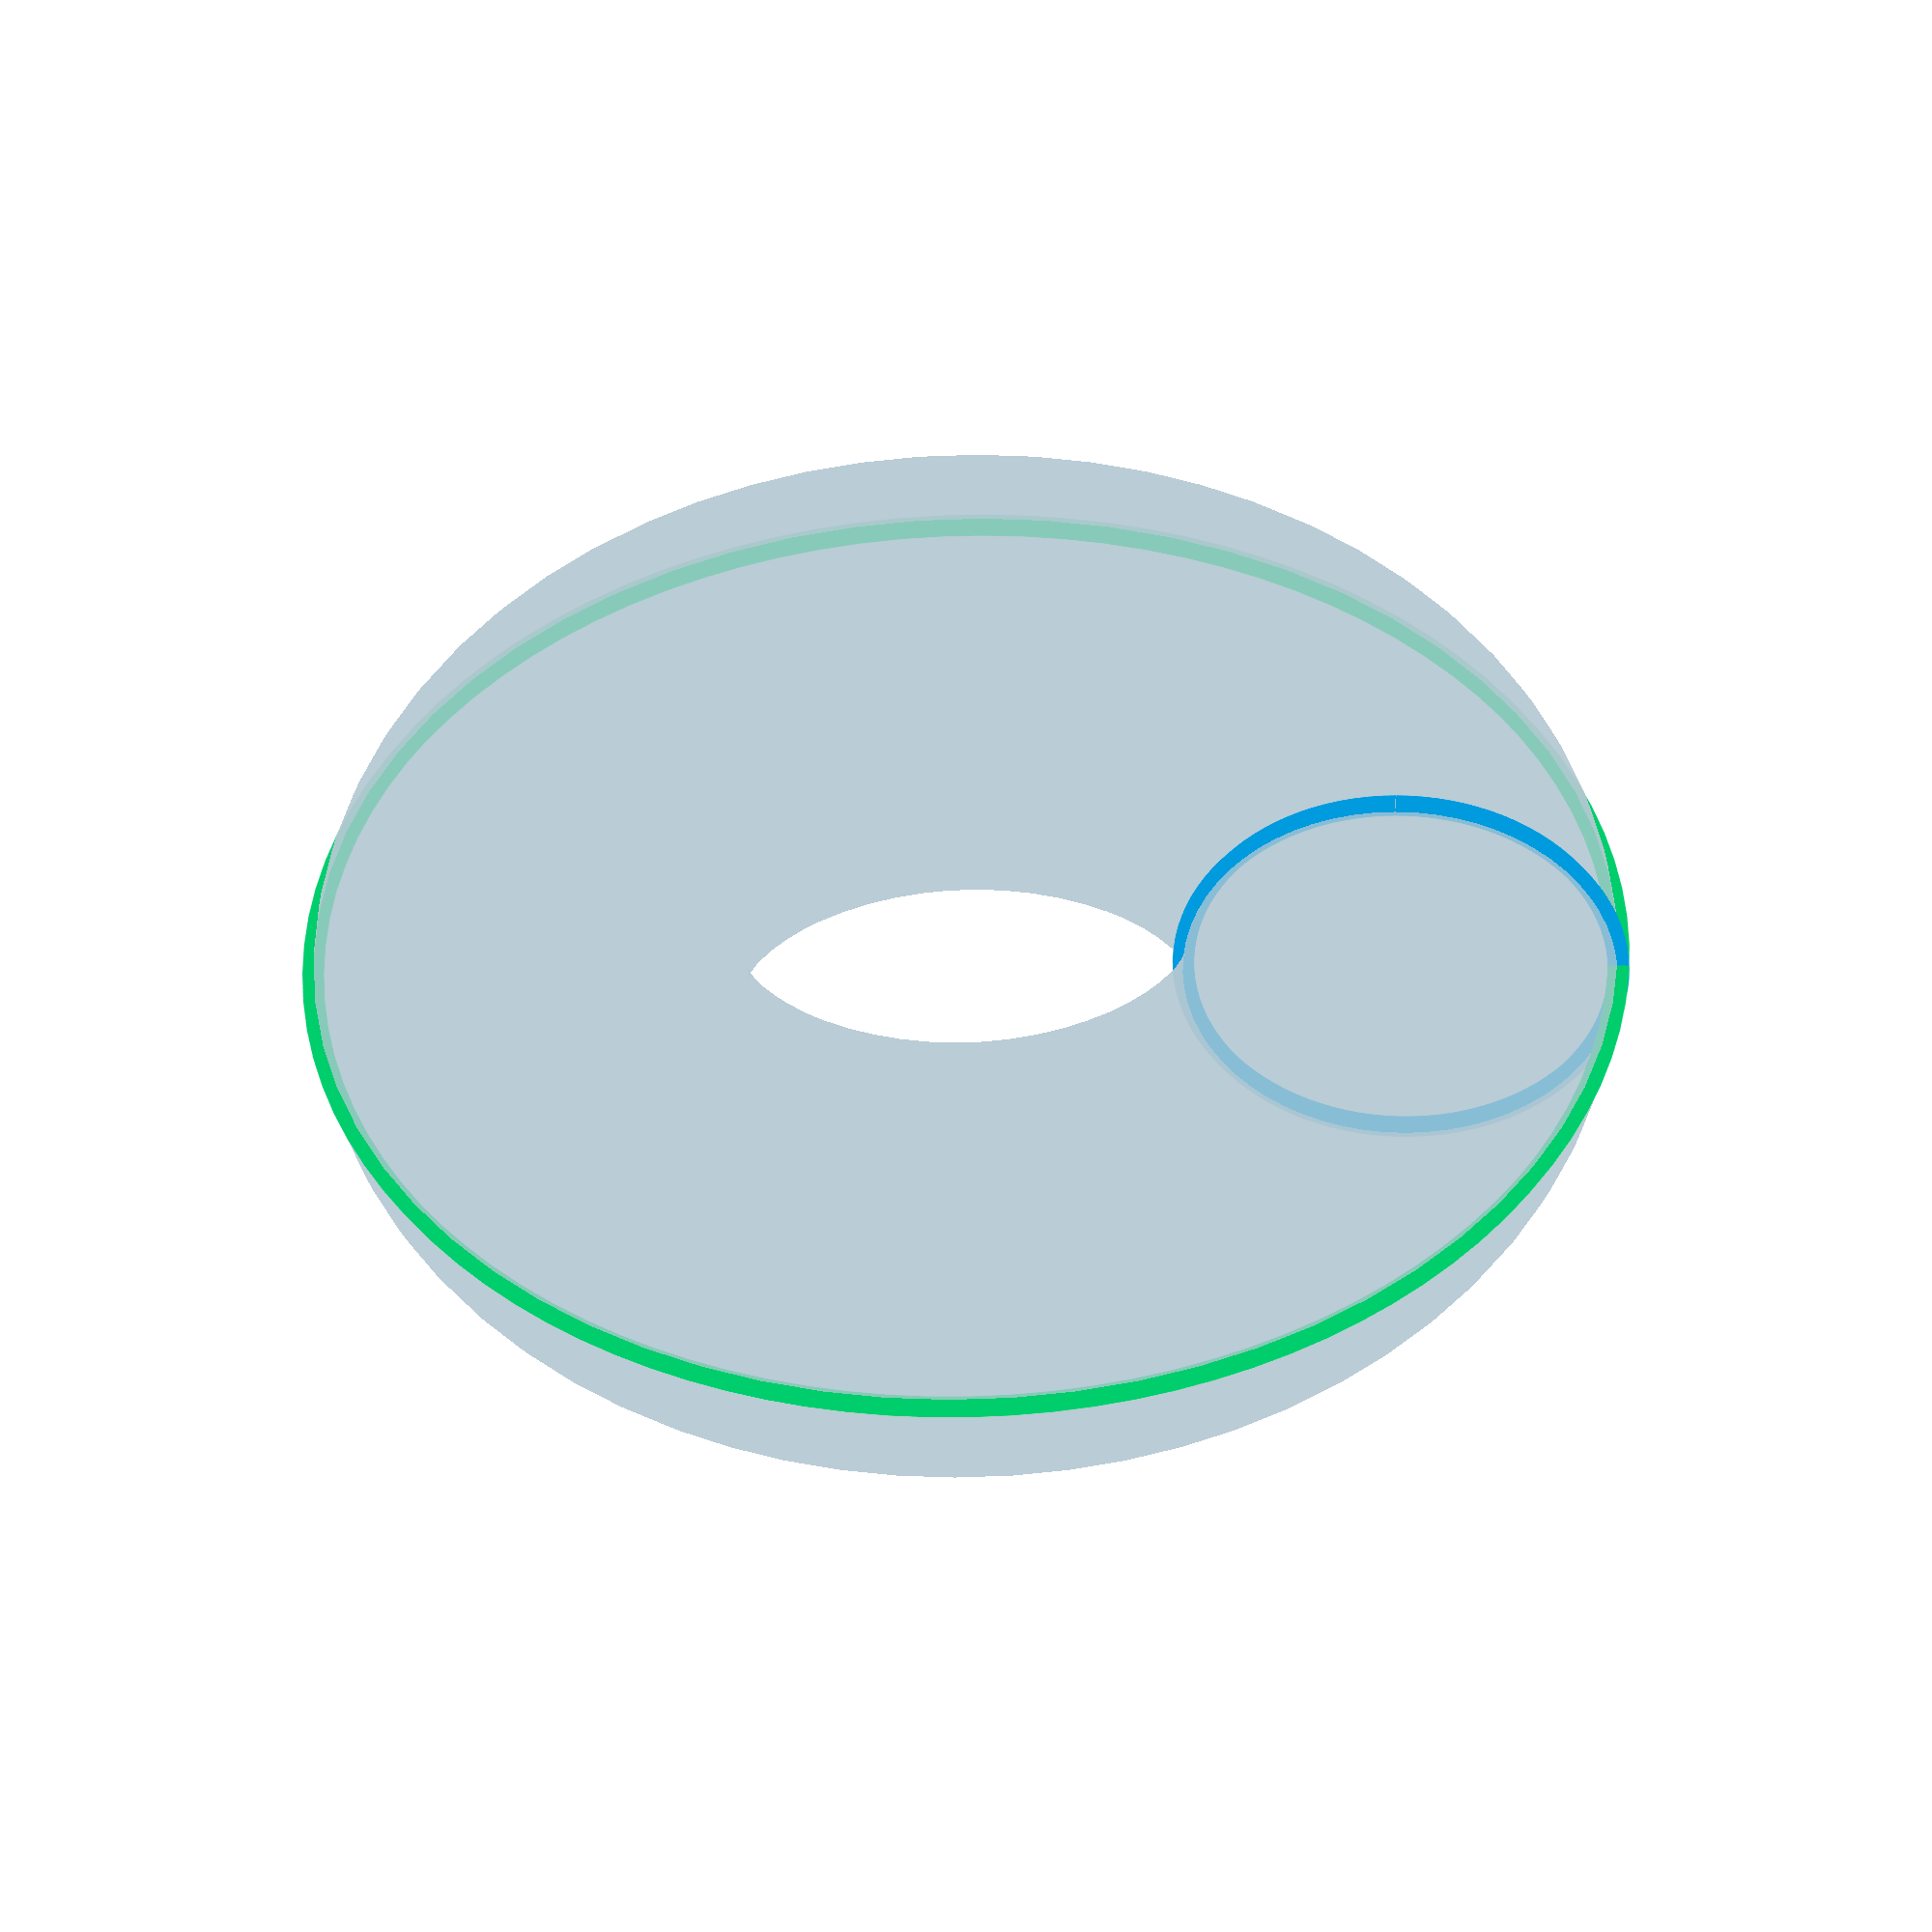
\includegraphics[trim=0 300 0 300, clip, width=0.4\textwidth]{figures/torus2}
  \caption{A torus and two representative cycles in $\hom_1$. (Right) a homologous cycle.}\label{fig:torus}
\end{figure}

\paragraph{Relative Homology}

Let $(X, Y)$ be a pair of topological spaces (or pair of simplicial complexes).
The relative chain groups $C_k(X, Y) = C_k(X) / C_k(Y)$ consist of equivalence classes of chains in $C_k(X)$ that differ by chains in $C_k(Y)$.
We note that the boundary map $\partial_k$ on $C_k(X)$ induces a boundary map on the quotient $C_k(X, Y)$ such that $\partial_k(y) = 0$ for all $y\in C_k(Y)$.

The \textbf{$k$th relative homology group} $\hom_k(X, Y)$ consists of homology classes of relative cycles---chains in $C_k(X)$ whose boundaries vanish or lie in $Y$.
That is, a relative $k$-cycle can either be a cycle in $C_k(X)$ or a chain in $C_k(X)$ with a boundary in $C_{k-1}(Y)$.
We will make extensive use of the \textbf{excision} axiom of homology which states that for any $A\subset Y$ such that $\cl_X(A)\subseteq \intr_X(Y)$ the inclusion of pairs $(X\setminus A, Y\setminus A)\hookrightarrow (X, Y)$ induces isomorphisms on relative homology groups $\hom_k(X\setminus A, Y\setminus A)\cong\hom_k(X, Y)$.

% \paragraph{Exact Sequences}
%
% A sequence $A\xrightarrow{i} B\xrightarrow{j} C$ is said to be \textbf{exact} if $\im~i = \ker~j$.
% An exact sequence $0\to A\to B\to C\to 0$ is said to be \textbf{short exact}.
% In general, any exact sequence $\ldots\to A\to B\to C\to\ldots$ is referred to as a long exact sequence.
%
% For any pair of topological spaces $(X, Y)$ the \textbf{long exact sequence of the pair} is the exact sequence
% \[ \ldots\to\hom_{k+1}(X, Y)\xrightarrow{\partial_{k+1}} \hom_k(Y)\xrightarrow{i_k} \hom_k(X)\xrightarrow{j_k}\hom_k(X, Y)\xrightarrow{\partial_k}\hom_{k-1}(Y)\to\ldots.\]
% Here the map $\partial_k$ is the connecting homomorphism which is induced by the boundary map on $C_k(X, Y)$.

% section homology (end)
